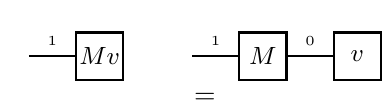
\begin{tikzpicture}[scale=0.3,thick] % , baseline = -3.5pt
    \draw (-7,2)--(-5,2) node[midway,above] {\tiny $\catvariableof{1}$};
    \draw (-5,1) rectangle (-3,3);
    \node[anchor=center] (text) at (-4,2) {\small $Mv$};

    \drawtextnode{-2}{2}{${=}$}

    \draw (-1,2)--(1,2) node[midway,above] {\tiny $\catvariableof{1}$};
    \draw (1,1) rectangle (3,3);
    \node[anchor=center] (text) at (2,2) {\small $M$};
    \draw (3,2)--(5,2) node[midway,above] {\tiny $\catvariableof{0}$};

    \draw (5,1) rectangle (7,3);
    \node[anchor=center] (text) at (6,2) {\small $v$};
%    \draw (7,2)--(9,2) node[midway,above] {\tiny $\catvariableof{0}$};
\end{tikzpicture}